% Options for packages loaded elsewhere
\PassOptionsToPackage{unicode}{hyperref}
\PassOptionsToPackage{hyphens}{url}
\PassOptionsToPackage{dvipsnames,svgnames,x11names}{xcolor}
%
\documentclass[
  letterpaper,
  DIV=11,
  numbers=noendperiod]{scrartcl}

\usepackage{amsmath,amssymb}
\usepackage{iftex}
\ifPDFTeX
  \usepackage[T1]{fontenc}
  \usepackage[utf8]{inputenc}
  \usepackage{textcomp} % provide euro and other symbols
\else % if luatex or xetex
  \usepackage{unicode-math}
  \defaultfontfeatures{Scale=MatchLowercase}
  \defaultfontfeatures[\rmfamily]{Ligatures=TeX,Scale=1}
\fi
\usepackage{lmodern}
\ifPDFTeX\else  
    % xetex/luatex font selection
\fi
% Use upquote if available, for straight quotes in verbatim environments
\IfFileExists{upquote.sty}{\usepackage{upquote}}{}
\IfFileExists{microtype.sty}{% use microtype if available
  \usepackage[]{microtype}
  \UseMicrotypeSet[protrusion]{basicmath} % disable protrusion for tt fonts
}{}
\makeatletter
\@ifundefined{KOMAClassName}{% if non-KOMA class
  \IfFileExists{parskip.sty}{%
    \usepackage{parskip}
  }{% else
    \setlength{\parindent}{0pt}
    \setlength{\parskip}{6pt plus 2pt minus 1pt}}
}{% if KOMA class
  \KOMAoptions{parskip=half}}
\makeatother
\usepackage{xcolor}
\setlength{\emergencystretch}{3em} % prevent overfull lines
\setcounter{secnumdepth}{-\maxdimen} % remove section numbering
% Make \paragraph and \subparagraph free-standing
\ifx\paragraph\undefined\else
  \let\oldparagraph\paragraph
  \renewcommand{\paragraph}[1]{\oldparagraph{#1}\mbox{}}
\fi
\ifx\subparagraph\undefined\else
  \let\oldsubparagraph\subparagraph
  \renewcommand{\subparagraph}[1]{\oldsubparagraph{#1}\mbox{}}
\fi


\providecommand{\tightlist}{%
  \setlength{\itemsep}{0pt}\setlength{\parskip}{0pt}}\usepackage{longtable,booktabs,array}
\usepackage{calc} % for calculating minipage widths
% Correct order of tables after \paragraph or \subparagraph
\usepackage{etoolbox}
\makeatletter
\patchcmd\longtable{\par}{\if@noskipsec\mbox{}\fi\par}{}{}
\makeatother
% Allow footnotes in longtable head/foot
\IfFileExists{footnotehyper.sty}{\usepackage{footnotehyper}}{\usepackage{footnote}}
\makesavenoteenv{longtable}
\usepackage{graphicx}
\makeatletter
\def\maxwidth{\ifdim\Gin@nat@width>\linewidth\linewidth\else\Gin@nat@width\fi}
\def\maxheight{\ifdim\Gin@nat@height>\textheight\textheight\else\Gin@nat@height\fi}
\makeatother
% Scale images if necessary, so that they will not overflow the page
% margins by default, and it is still possible to overwrite the defaults
% using explicit options in \includegraphics[width, height, ...]{}
\setkeys{Gin}{width=\maxwidth,height=\maxheight,keepaspectratio}
% Set default figure placement to htbp
\makeatletter
\def\fps@figure{htbp}
\makeatother

\KOMAoption{captions}{tableheading}
\makeatletter
\makeatother
\makeatletter
\makeatother
\makeatletter
\@ifpackageloaded{caption}{}{\usepackage{caption}}
\AtBeginDocument{%
\ifdefined\contentsname
  \renewcommand*\contentsname{Table of contents}
\else
  \newcommand\contentsname{Table of contents}
\fi
\ifdefined\listfigurename
  \renewcommand*\listfigurename{List of Figures}
\else
  \newcommand\listfigurename{List of Figures}
\fi
\ifdefined\listtablename
  \renewcommand*\listtablename{List of Tables}
\else
  \newcommand\listtablename{List of Tables}
\fi
\ifdefined\figurename
  \renewcommand*\figurename{Figure}
\else
  \newcommand\figurename{Figure}
\fi
\ifdefined\tablename
  \renewcommand*\tablename{Table}
\else
  \newcommand\tablename{Table}
\fi
}
\@ifpackageloaded{float}{}{\usepackage{float}}
\floatstyle{ruled}
\@ifundefined{c@chapter}{\newfloat{codelisting}{h}{lop}}{\newfloat{codelisting}{h}{lop}[chapter]}
\floatname{codelisting}{Listing}
\newcommand*\listoflistings{\listof{codelisting}{List of Listings}}
\makeatother
\makeatletter
\@ifpackageloaded{caption}{}{\usepackage{caption}}
\@ifpackageloaded{subcaption}{}{\usepackage{subcaption}}
\makeatother
\makeatletter
\@ifpackageloaded{tcolorbox}{}{\usepackage[skins,breakable]{tcolorbox}}
\makeatother
\makeatletter
\@ifundefined{shadecolor}{\definecolor{shadecolor}{rgb}{.97, .97, .97}}
\makeatother
\makeatletter
\makeatother
\makeatletter
\makeatother
\ifLuaTeX
  \usepackage{selnolig}  % disable illegal ligatures
\fi
\IfFileExists{bookmark.sty}{\usepackage{bookmark}}{\usepackage{hyperref}}
\IfFileExists{xurl.sty}{\usepackage{xurl}}{} % add URL line breaks if available
\urlstyle{same} % disable monospaced font for URLs
\hypersetup{
  pdftitle={Predicting Rocket League Game Outcome Through Statistical Modeling},
  colorlinks=true,
  linkcolor={blue},
  filecolor={Maroon},
  citecolor={Blue},
  urlcolor={Blue},
  pdfcreator={LaTeX via pandoc}}

\title{Predicting Rocket League Game Outcome Through Statistical
Modeling}
\author{}
\date{}

\begin{document}
\maketitle
\ifdefined\Shaded\renewenvironment{Shaded}{\begin{tcolorbox}[sharp corners, enhanced, frame hidden, interior hidden, borderline west={3pt}{0pt}{shadecolor}, boxrule=0pt, breakable]}{\end{tcolorbox}}\fi

\linenumbers

\textbf{Project Introduction:}

Over the past decade, the world of esports and competitive video-gaming
has seen a drastic boom in popularity. One of the most popular esports
is Rocket League, which is essentially soccer played in cars. I am a fan
of professional Rocket League, and I also have played the video game
competitively as a member of the esports team at St.~Lawrence
University.

Rocket League is a video game that can be played on a PC, Xbox,
PlayStation, and Nintendo Switch. Much like regular soccer, there is one
ball and two goals, and you win by scoring more goals than your
opponent. The game is played with a randomly assigned ``blue'' and
``orange'' team, and each player controls one rocket-powered car. There
are different game modes within the game, but for the purposes of this
project I will be focusing on the 3v3 game-mode, which is where the
majority of competitive play occurs and is also the mode where most of
the competitive cash prizes are. Rocket League was released by Psyonix
on July 7th, 2015.

Despite being released in 2015, the competitive and professional side of
the video game is still growing to this day. In 2022, the total prize
pool given out by Psyonix alone reached \$6,000,000, and there are other
non-Psyonix hosted tournaments with cash prizes as well. This past year
the video game has expanded to new regions, including Asia-Pacific
North, Asia-Pacific South, and Middle East/North Africa. Players are
constantly pushing the skill ceiling to re-define what it means to be
the best in the world. With these improvements come constantly changing
strategy and tactics that make for an even more thrilling viewer
experience.

Much like with popular sports such as baseball and football, there is a
growing analytical side for assessing performance of some of the most
popular esports. These are used to help strategize, coach, and improve
competitive gamers' performances. While analytics are useful to some
competitive video games, Rocket League is a relatively new esport, and
the statistical side of the game is widely unexplored. As both a fan and
a player of Rocket League, and somebody with an interest in statistics
and data science in general, I was curious to see if statistical
learning algorithms could be applied to predicting game outcomes. These
findings could potentially help form different strategies among
professional teams and could even help coaches to decide what areas to
put more of a focus on going into games.

\textbf{Introduction to Dataset/Variables:}

For this project, I only explored the three player vs.~three player
game-mode and looked at a dataset collected on the main professional
competition that runs throughout the year; RLCS (Rocket League
Championship Series). All of the data was obtained using octane.gg and
ballchasing.com and spans over the course of multiple RLCS events
throughout the 2021-2022 season. The dataset includes information on the
teams in the match, team statistics (such as saves, assists, shots,
etc.), boost statistics (boost used, boost stolen, time spent without
boost, etc.), and movement statistics (time spent moving slow, time
spent in each team's half, time spent in air, etc.). Each game in the
dataset had two rows, one for the statistics for the blue team and one
for the statistics of the orange team.

Using this dataset, I calculated net variables by subtracting all of the
blue team's stats from all of the orange team's stats. This allowed me
to see the variables where having more or less than the opponent would
be positively associated with winning. (For instance, examining whether
a team's chances of winning a match increased if they recorded more or
less saves than their opponent.) I utilized a Random Forest model
approach in order to try and predict whether teams would win/lose their
match based on the net variables in the dataset.

Additionally, I wanted to investigate whether or not different team play
styles were consistently associated with winning/losing. To tackle this
task, I used a dataset of individual player statistics on the same
matches that I had used for team data. I wanted to see if teams who had
certain players in different roles performed noticeably better/worse
than teams who didn't play very positionally. (If one team had a
``goalie'' player, his saves would be noticeably higher than his
teammates, a ``goal-scorer'' would have higher shots and goals than his
teammates, etc.). To tackle this task, within each game for each team I
calculated standard deviation variables for all of the variables in the
dataset and also calculated the difference by blue team - orange team.

Here's an example of what core\_shots\_diff and sd\_core\_shots\_diff
would look like for a given game. Let's say the players on the blue team
recorded 4 shots, 3 shots, and 2 shots respectively. Let's also say the
players on the orange team recorded 6 shots, 5 shots, and 1 shot
respectively. Then, the total shots would be 9 for blue and 12 for
orange, so the \emph{core\_shots\_diff} would be \emph{-3}. (Always
calculated as blue team - orange team to remain consistent). The
standard deviation for the blue team would be roughly 0.82, and the
standard deviation for the orange team would be roughly 2.16. Then, the
\emph{sd\_core\_shots\_diff} would be 0.82 - 2.16 = \emph{-1.34} for
that game.

\textbf{Investigative Plots:} Before creating any models to try to
predict game outcome, I did some exploratory plotting of different
individual variables in order to get an idea of what variables may have
strong correlation with winning games. Unfortunately, out of all of the
variables that I investigated, the majority did not appear to have a
strong correlation with winning games. However, there were some
interesting observations that I made; one in particular that surprised
me was that movement speed appears to have little to no correlation to
match outcome. As a player myself, we are always coached that keeping
your speed as high as possible around the field is vital in order to
become a high level player. But, in this dataset of only professional
matches, that does not appear to be the case.

Two variables to note that provided some clear correlation to game
outcome were ``core\_shots\_diff'' (difference in shots taken between
the two teams), and ``positioning\_time\_behind\_ball\_diff''
(difference in the amount of time each team spent goal side of the
ball).

\textbf{core\_shots\_diff plotted against winner:}

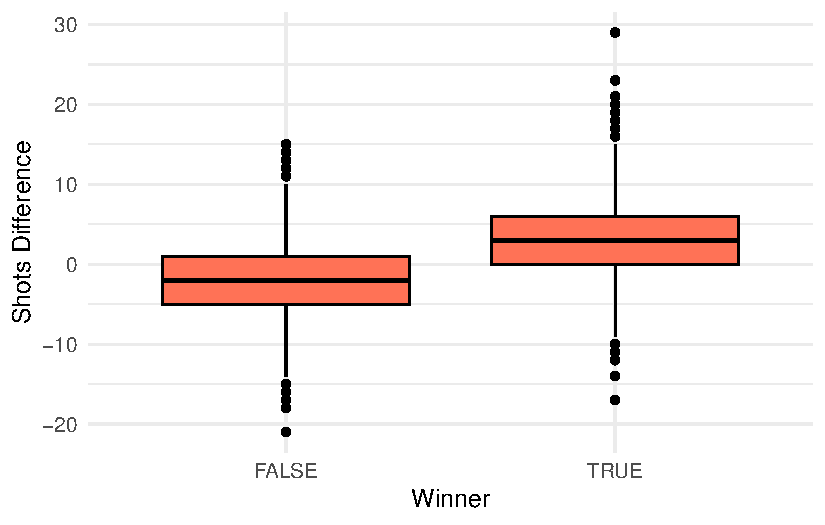
\includegraphics{RL_Write_Up_files/figure-pdf/unnamed-chunk-2-1.pdf}

\textbf{postioning\_time\_behind\_ball\_diff plotted against winner:}

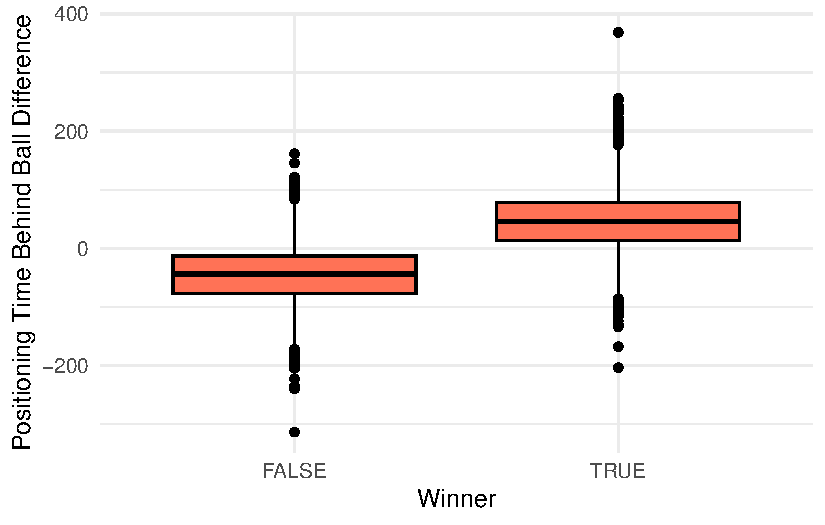
\includegraphics{RL_Write_Up_files/figure-pdf/unnamed-chunk-3-1.pdf}

I was surprised to find such a clear correlation between spending more
time behind the ball being so positively associated with winning games.
But, it does make sense that if the ball spends more time near your
opponent's goal rather than your goal, that would lead to positive
results.

\textbf{Methods:}

As I mentioned previously, for this project I used a random forest
statistical modeling approach. A random forest model is a type of
statistical learning method that combines ``decision trees'' in order to
make a prediction. Each tree is made up of a random subset of predictor
variables from the full dataset. The predictions from each of these
decision trees are combined to make one final prediction for each
observation.

The random forest approach can be used for two main purposes:
classification or regression. Since the goal of my model was to classify
games as wins or losses, I used the classification approach.

I started my Random Forest model by making a random train/test split of
the data. However, in case there was any chance that the model was
yielding higher results because certain series were partially in the
training dataset and partially in the test dataset, I created a
series\_id variable by combining the names of the two teams in the
series. When I did my train/test data split, I grouped by series\_id so
that every series would be entirely in the train set or entirely in the
test set.

An important element of the random forest approach is bootstrapping.
Bootstrapping is essentially sampling the set-aside training data with
replacement to create many different simulated samples. This process is
useful for understanding bias and variance present within the dataset.
(Kaggle source)

The random forest approach also makes use of bagging when creating its
model. Bagging starts with creating different training subsets with
replacement randomly (bootstrapping).(simplilearn source) Then, a base
model is created and fit to each of these subsets of the training data.
These models run independently of each other, and final predictions are
determined by combining the predictions from all of the models. (Kaggle
source) Bagging is one of the advantages of random forest models,
because it reduces variations in predictions in the process of combining
the results of multiple decision trees on different samples of the
training data. (edureka source)

Plot that demonstrates bootstrapping and bagging process:

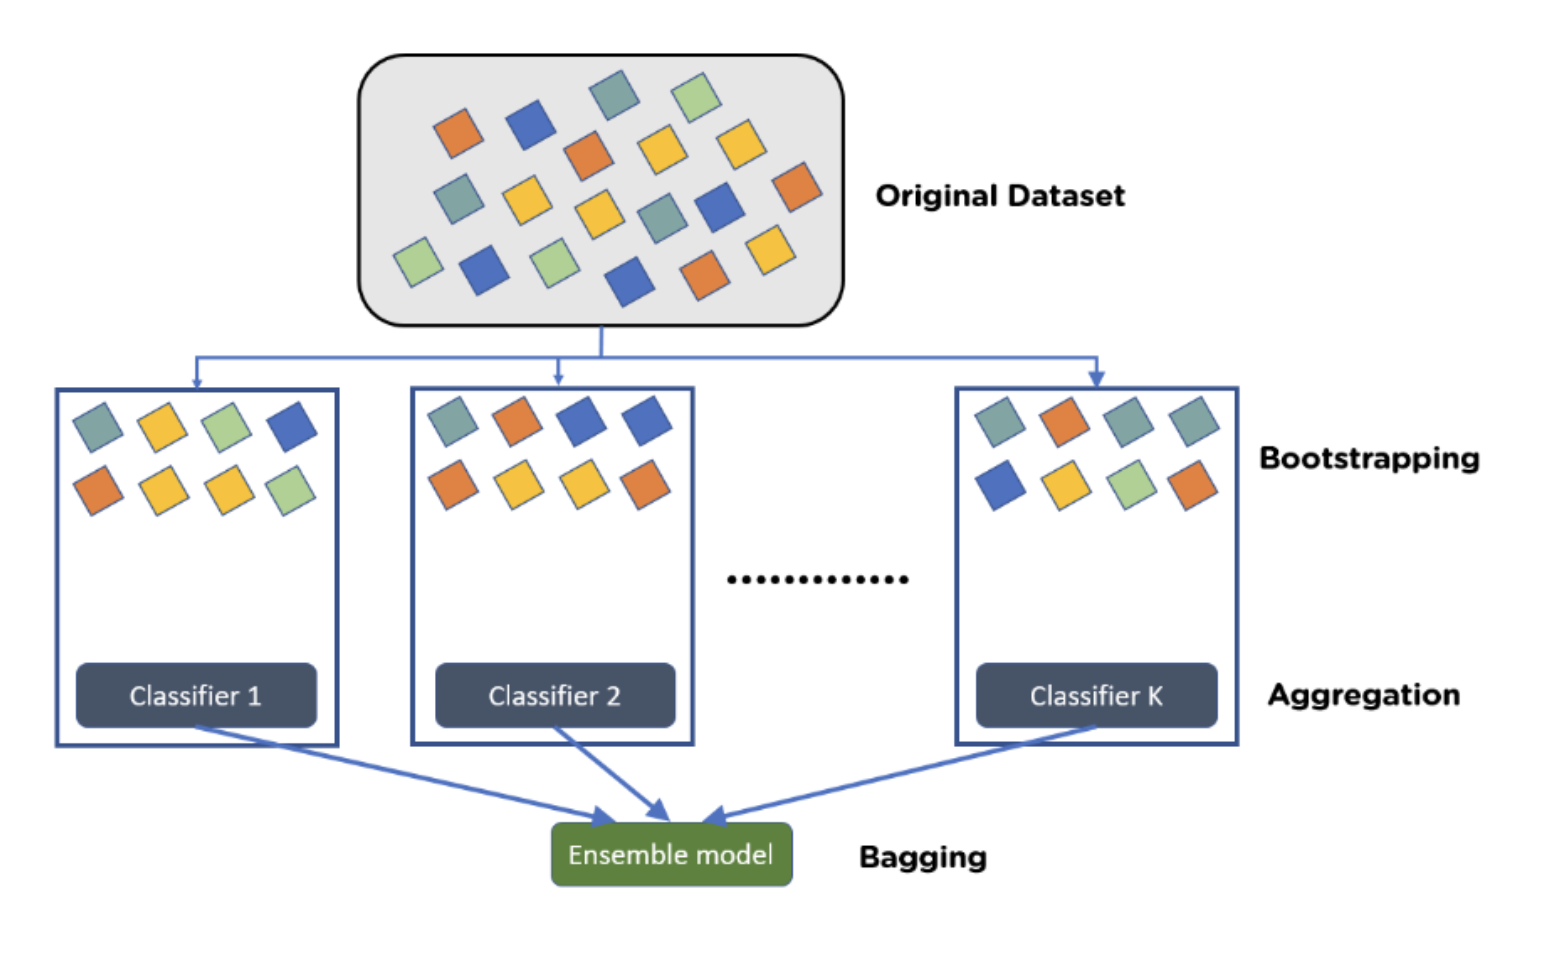
\includegraphics{../Images/Bootstrapping_Bagging_img.png}

\textbf{Random Forest Results:}

Utilizing the full dataset with all of the net variables as well as all
of the standard deviation difference variables, I created a random
forest model to predict the winner of each game. Using this random
forest model that was trained on the training data, we then tested the
model on the test data in order to analyze how strong the model was. The
final step in this process was to get predictions on the game outcome of
all the games in the RL\_test dataset, and see how accurately the model
performed:

\begin{verbatim}
          Truth
Prediction    1    0
         1 4615  764
         0  510 2850
\end{verbatim}

The model predicted 4615 true positives, 2850 true negatives, 764 false
positives, and 510 false negatives. This combines for a total
classification accuracy of 85.422\%.

Below is an example of a single decision tree that utilizes the
variables boost\_time\_zero\_boost\_diff (difference in the amount of
time each team's players spent without any boost) and
positioning\_time\_offensive\_half\_diff (the difference in the amount
of time each team spent in the offensive half). In this example, the
tree analyzes whether the difference in the time at zero boost is
greater or less than 0.8. If it is greater than a 0.8 difference, it
then looks to see if the difference in the amount of time spent in the
offensive half between the two teams is more or less than 22 before
making its prediction.

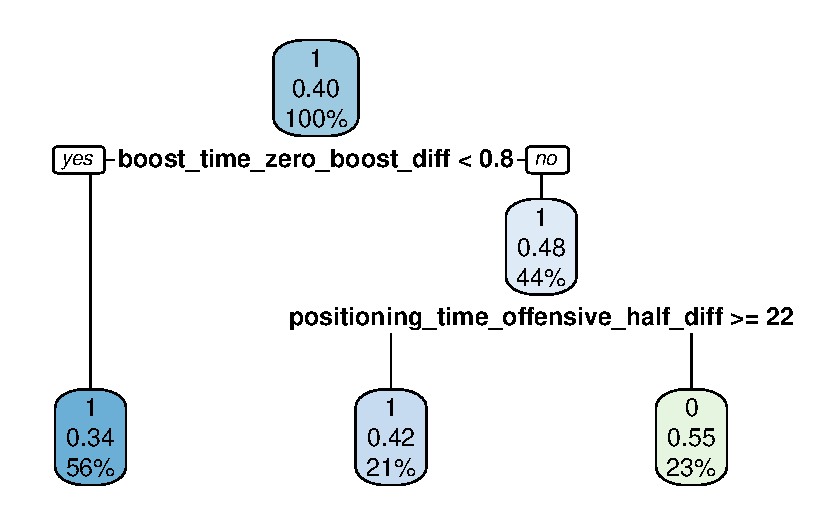
\includegraphics{RL_Write_Up_files/figure-pdf/unnamed-chunk-6-1.pdf}

A variable importance plot provides a way to analyze the significance of
each of the predictors utilized in the random forest model. Below is a
variable importance plot that shows the 10 most ``important'' variables
to my random forest model:

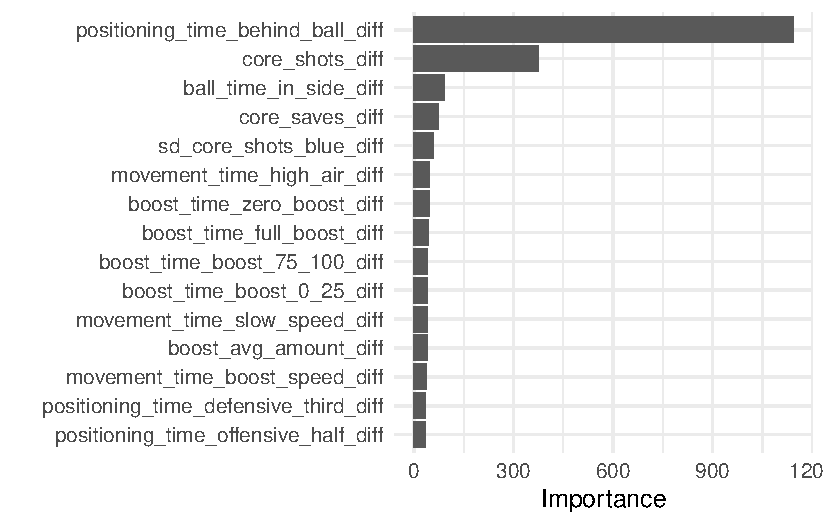
\includegraphics{RL_Write_Up_files/figure-pdf/unnamed-chunk-7-1.pdf}

The clear strongest variable in the model was the difference in teams'
positioning time behind the ball. The difference in shots taken also
proved to be a strong predictor in determining game outcome.

\textbf{Conclusion:}

Through exploratory plots and multiple random forest models built, there
were an unmistakable two predictors that were stronger than the rest.
These variables were the difference in shots taken and the difference in
time spent behind (or goalside) of the ball. It can be surprising at
first that more time spent goal side of the ball provides such a strong
chance of winning the game, but from a strategical standpoint it
actually makes sense.

One of the most common tactics in Rocket League that is also prominent
in other sports is putting constant pressure on the opposing team. If
you are constantly putting the team under pressure, the ball is going to
constantly be in the opposing team's defensive half, and they probably
will be conceding a lot of shots. If the ball is always in the opposing
team's half, you are far more likely to be goalside of the ball, and you
are also likely to be the team that got more shots off.

One of the most common things you'll hear from players and coaches if
you are a fan of Rocket League is that you should be making an effort to
keep your car's speed/momentum high as much as possible throughout the
course of the game. Interestingly, there were many variables related to
movement speed, and almost none of them were significant predictors at
all. The most significant movement variable towards predicting game
outcome was movement\_time\_slow\_speed\_diff (the difference in the
amount of time each team's cars spent moving slow), but even this was
not a particularly strong predictor.

One potential explanation for this is that once you reach a high enough
level, every player is moving so fast the whole time and every player is
capable of playing well while moving fast, that it becomes less of a
strategic advantage than it is at some lower ranks in the game. It's
entirely possible that for non-professional level players, this is still
an extremely important factor, but once you reach a high enough skill
level it almost doesn't make a difference.

Another interesting finding through this model was that almost none of
the team standard deviation differences proved to be significant
predictors. This means that through this model alone, we cannot
determine whether different strategies



\end{document}
